%%This is a very basic article template.
%%There is just one section and two subsections.
\documentclass[a4paper,11pt]{scrartcl}
\usepackage{polski}
\usepackage[utf8]{inputenc}
\usepackage[T1]{fontenc}
\usepackage{datetime}

\usepackage{listings}
\usepackage{graphicx, graphics, epsfig, geometry, pslatex}
\usepackage{amsmath, amssymb}
\usepackage{url}

\usepackage{array}
\usepackage{times}
%\usepackage{fullpage}
\usepackage{caption}

\newcommand{\figsource}[1]{
\captionsetup{font={scriptsize, it}}
\caption*{Źródło: \url{#1}}
\captionsetup{font={normalsize}}
}

\newcommand{\f}{\texttt}
\newcommand{\mytitlea}{Peer-to-peer web objects}
\newcommand{\mytitleb}{caching proxy}
\newcommand{\me}{Tomasz Drwięga}
\newcommand{\s}{ }

\newcommand{\kesz}{cache}
\newcommand{\keszy}{cache'y}
\newcommand{\kesza}{cache'a}
\newcommand{\keszowi}{cache'owi}
\newcommand{\keszem}{cache'em}
\newcommand{\keszu}{cache'u}
\newcommand{\keszujace}{cache'ujące}
\newcommand{\keszujacego}{cache'ującego}
\newcommand{\keszujacy}{cache'ujący}
\newcommand{\keszujacym}{cache'ującym}
\newcommand{\keszujacych}{cache'ujących}
\newcommand{\keszowania}{cache'owania}
\newcommand{\keszowaniem}{cache'owaniem}

\lstset{numbers=left,
	numberstyle=\tiny,
	%basicstyle=\footnotesize,
	showstringspaces=false,
	basicstyle=\footnotesize,
	breaklines=true,
	captionpos=b,
	tabsize=3,
	stepnumber=60,
	firstnumber=1,
	}
%opening
\title{\mytitlea \mytitleb}
\author{\me}

\makeindex

\begin{document}

% \parindent0pt
\pagestyle{empty}

\begin{titlepage}
\vspace*{\fill}
\begin{center}
\begin{picture}(300,510)
	\put( 0,520){\makebox(0,0)[l]{\large \bf \textsc{Wydział Podstawowych
	Problemów Techniki}}}
	\put( 0,500){\makebox(0,0)[l]{\large \bf \textsc{Politechniki Wrocławskiej}}}
	\put(15,280){\makebox(0,0)[l]{\Huge  \bf \textsc{\mytitlea}}}
	\put(80,250){\makebox(0,0)[l]{\Huge  \bf \textsc{\mytitleb}}}
	\put(95,220){\makebox(0,0)[l]{\Large     \textsc{\me}}}
	
	\put(190, 80){\makebox(0,0)[l]{\large  {Praca magisterska napisana}}}
	\put(190, 60){\makebox(0,0)[l]{\large  {pod kierunkiem}}}
	\put(190, 40){\makebox(0,0)[l]{\large  {dra Mirosława Korzeniowskiego}}}
	
	\put(110,-80){\makebox(0,0)[bl]{\large \bf \textsc{Wrocław 2013}}}
\end{picture}
\end{center}
\vspace*{\fill}
\end{titlepage}

\tableofcontents

\newpage

\pagestyle{headings}

\section*{Wstęp}

TODO: Opis problemu cachowania (oryginalnego - hot spots), nasilenie związane z efektem slashdot, multimedia

\section{Historia \keszowania}
Wraz z rosnącą liczbą użytkowników Internetu w latach dziewięćdziesiątych zaczęły pojawiać się problemy z dostępem do pewnych zasobów.
Duża liczba odwołań do popularnych strony, w krótkim czasie powodowała znaczące obciążenie serwerów, które dany zasób posiadały.
Czasami z powodu nadmiernego zalania\footnote{ang. \textit{flooded}, \textit{swamped}} żądaniami serwer nie był w stanie obsłużyć wszystkich, przez co strona stawała się niedostępna.

\subsection{Serwery \keszujace}\label{sect_cache}
Jako rozwiązanie problemu ,,gorących punktów'' (ang. \textit{hot spots}) pojawiły się serwery \keszujace. Rysunek \ref{fig_cache_server} przedstawia wprowadzenie transparentnego, lokalnego \kesza\s i jego relację z serwerem docelowym. 
Żądania zasobów wychodzące od użytkowników końcowych są w pierwszej kolejności obsługiwane przez serwer \keszujacy, który odpowiada zapamiętanym zasobem lub kontaktuje się z serwerem docelowym i zapamiętuje odpowiedź.

\begin{figure}[ht]
\centering
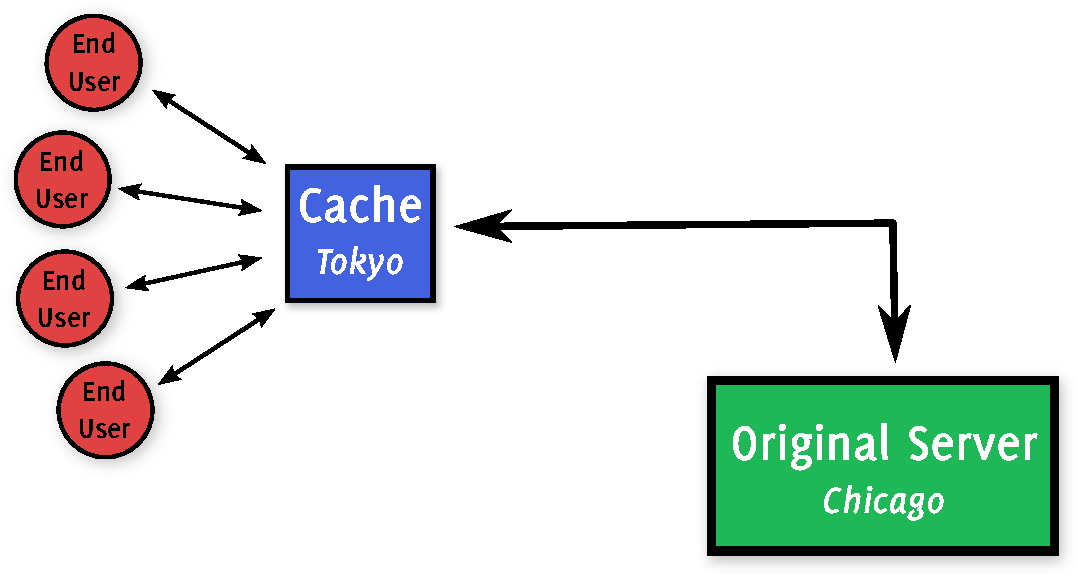
\includegraphics[width=0.85\linewidth]{img/cache.pdf}
\caption{
Przykład lokalnego serwera \keszujacego.
Zamiast wielokrotnie odwoływać się do docelowego serwera, który zawiera daną stronę
możemy zapamiętać ją na serwerze \keszujacym. Takie rozwiązanie niesie ze sobą zalety
zarówno dla administratorów serwera w Chicago, jak i użytkowników sieci w Japonii:
mniej żądań skutkuje mniejszym obciążeniem serwera, a ,,lokalność'' serwera \keszujacego\s zmniejsza opóźnienia i zwiększa szybkość transferu zasobu.
}
\label{fig_cache_server}
\end{figure}

Wprowadzenie \keszowania\s niesie ze sobą szereg zalet nie tylko dla administratorów serwerów zawierających zasoby. Serwery znajdujące się na granicy sieci lokalnej z Internetem (jak na rysunku \ref{fig_cache_server}) oferują użytkownikom tej sieci lepszy transfer i mniejsze opóźnienia w dostępie do popularnych zasobów.
Ponieważ łącze wychodzące z sieci ma ograniczoną przepustowość, \kesz\s pozwala również na jego oszczędniejsze wykorzystanie, a tym samym poprawę jakości dostępu do Internetu.

\subsection{Rozproszony i hierarchiczny \kesz}\label{sect_dist_cache}
Rozwiązanie przedstawione w rozdziale \ref{sect_cache} pozwala na odciążenie serwera docelowego. Zastanówmy się jednak co będzie się działo w przypadku zwiększania liczby użytkowników korzystających z serwera \keszujacego. Duża liczba żądań może spowodować dokładnie taką samą sytuację jak w przypadku serwera docelowego - \kesz\s zostanie zalany i nie będzie w stanie obsłużyć wszystkich zapytań.

W 1995 roku Malpani i inni \cite{malpani1995making} zaproponowali metodę, w której wiele serwerów \keszujacych\s współpracuje ze sobą w celu zrównoważenia obciążenia. W ich propozycji klient wysyła żądanie do losowego serwera należącego do systemu. W przypadku, gdy serwer posiada określony zasób odsyła go w odpowiedzi, w przeciwnym razie rozsyła to żądanie do wszystkich innych serwerów. Jeżeli żaden z \keszy nie zawiera zasobu, to żądanie jest przesyłane do serwera oryginalnego. Niestety wraz ze wzrostem liczby serwerów, należących do systemu liczba przesyłanych między nimi wiadomości bardzo szybko rośnie i cały system staje się zawodny.

W ramach projektu Harvest \cite{bowman1994harvest} A. Chankhunthod i inni \cite{chankhunthod1995hierarchical} stworzyli \kesz\s hierarchiczny. Rozwiązanie to pozwala łączyć kilka serwerów w system, który można skalować w zależności od liczby użytkowników, których ma obsługiwać. Grupy użytkowników łączą się z serwerami, będącymi liśćmi. Przychodzące żądania są obsługiwane najpierw przez serwery na najniższym poziomie, w przypadku gdy te serwery nie mają danego zasobu w \keszu\s decydują czy pobrać go z serwera docelowego, czy odpytać serwery z tego samego i wyższego poziomu. Decyzja podejmowana jest na podstawie opóźnień do obu serwerów.

\begin{figure}[h]
\centering
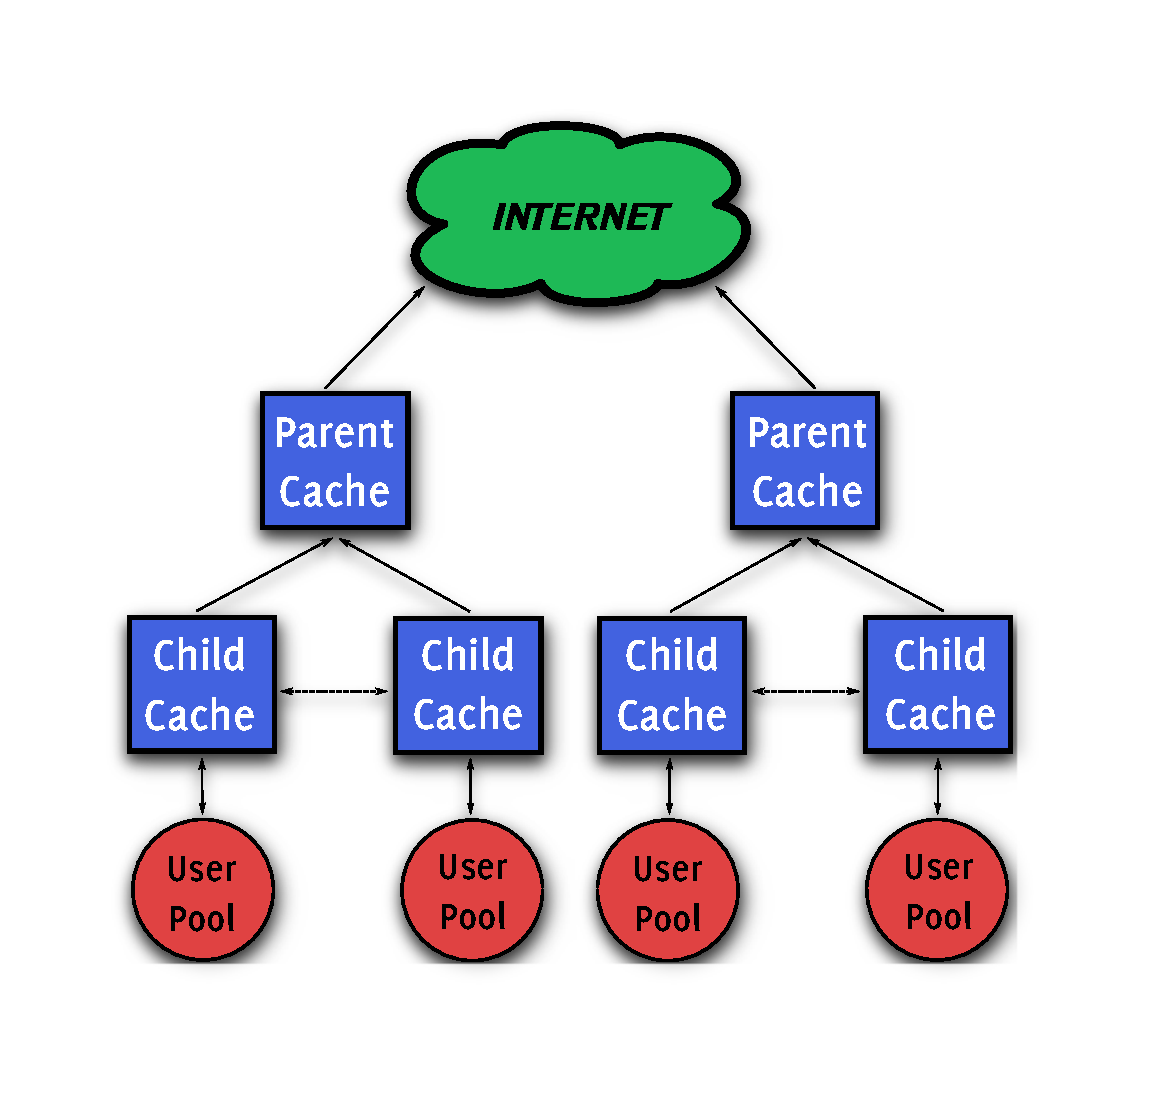
\includegraphics[width=0.8\linewidth]{img/hierarchical.pdf}
\label{fig_cache_hierarchical}
\caption{Połączenie kilu serwerów \keszujacych\s w system hierarchiczny. Każdy z serwerów znajdujących się w liściach obsługuje określoną liczbę użytkowników. Zapytania o zasoby, które nie znajdują się w \keszu\s wysyłane są do rodzica.}
\end{figure}

W praktyce, w takim systemie serwery na wyższych poziomach muszą obsługiwać dużą liczbę żądań od dzieci przez co stają się wrażliwe na zalanie oraz składują duże ilości danych \cite{povey1997distributed}.

Kolejnym zaproponowanym udoskonaleniem jest \kesz\s rozproszony. Rozwiązanie zachowuje hierarchiczną strukturę w formie drzewa, ale tym razem jedynie serwery w liściach zajmują się \keszowaniem\s zasobów, a pozostałe serwery stanowią indeks, w którym zapamiętywana jest informacja czy zasób znajduje się w systemie oraz jaki serwer go przechowuje.

Jak pokazały eksperymenty \cite{povey1997distributed} rozproszony \kesz\s oferuje zbliżoną wydajność do \keszu\s hierarchicznego rozwiązując dodatkowo problemy związane z obsługą dużej liczby żądań przez serwery na wyższych poziomach.

\subsection{Dynamiczna restrukturyzacja}
Przedstawione w rozdziałach \ref{sect_cache} i \ref{sect_dist_cache} metody \keszowania\s nie są przystosowane do działania w warunkach, w którym obciążenie czy liczba użytkowników obsługiwanych przez system się zmienia. Wraz z rosnącą liczbą żądań nie jest możliwe łatwe poprawienie wydajności przez dołożenie dodatkowych serwerów \keszujacych. Wprowadzenie zmian w systemie wymaga zmian w konfiguracji poszczególnych serwerów. Dodatkowo awarie pojedynczych węzłów mogą spowodować nieprawidłową pracę \keszu.

W celu ułatwienia dodawania i usuwania serwerów do systemu możemy spróbować innego podejścia do problemu. Podstawowym zadaniem węzłów wewnętrznych w systemie \keszu\s rozproszonego jest utrzymywanie indeksu przechowywanych zasobów i lokalizacja serwera, który dany zasób obsługuje. Zatem jeżeli klient mógłby określić, który serwer \keszujacy\s jest odpowiedzialny za obsługę obiektu, wtedy cała infrastruktura związana z indeksowaniem byłaby niepotrzebna.

Naiwnym rozwiązaniem stosującym takie podejście jest przypisanie zasobów do konkretnych serwerów. Przyjmijmy za identyfikator zasobu jego adres. Możemy teraz przypisać wszystkie zasoby w obrębie jednej domeny do pewnego serwera. Na przykład dysponując 24 serwerami możemy przypisać wszystkie domeny zaczynające się na ,,a'' do serwera pierwszego, na ,,b'' do drugiego itd. Oczywiście pozwoli to na łatwe określenie, który serwer należy odpytać o dany zasób, ale rozwiązanie to ma dwie poważne wady. Po pierwsze rozwiązanie nie jest skalowalne - niezdefiniowane jest jakie zasoby miałby obsługiwać dodatkowy serwer, a po drugie obciążenie na serwerach jest nierównomierne.

Możemy jednak spróbować rozwiązać problem przydziału zasobów do serwerów nieco inaczej. Niech $n$ oznacza liczbę serwerów, a $R$ adres pewnego zasobu, wtedy:
\begin{equation*}
S \equiv hash(R) \bmod n,
\end{equation*}
 gdzie $S$ oznacza indeks serwera odpowiedzialnego za zasób $R$, a $hash$ jest funkcją haszującą. Dzięki właściwościom funkcji haszujących gwarantujemy, że zasoby każdy z serwerów jest odpowiedzialny za równą część składowanych zasobów. Niestety dalej nie jest rozwiązany problem skalowalności. Dodanie $n+1$ serwera powoduje, że wszystkie zasoby zostaną przypisane w inne miejsca.
 
\subsubsection{\textit{Consistent Hashing}}
Podczas dodawania nowego serwera do systemu oczekujemy, że przejmie on od pozostałych równą część zasobów, aktualnie znajdujących się w \keszu. Dodatkowo nie chcemy, aby wartości w \keszu były przesuwane pomiędzy ,,starymi'' serwerami. Taką własność gwarantuje mechanizm \textit{Consistent Hashing}, opracowany przez Kargera i Lehmana \cite{karger1997consistent}.

Załóżmy, że dysponujemy funkcją haszującą w odcinek $[0, 1]$, za pomocą której każdemu zasobowi i serwerowi przyporządkowujemy punkt na tym odcinku. Dodatkowo, traktujemy odcinek jako okrąg o obwodzie równym 1. W podanym przez Kargera i Lehmana schemacie dany zasób jest obsługiwany przez najbliższy serwer idąc zgodnie z ruchem wskazówek zegara. Rysunek \ref{fig_consistent_hashing} przedstawia przykładowe mapowanie zasobów i ich przyporządkowanie do poszczególnych serwerów. W drugiej części rysunku przedstawiona została zmiana przyporządkowania wynikająca z dodania nowego serwera $D$.

\begin{figure}[ht]
\centering
\begin{minipage}[b]{0.445\linewidth}
\centering
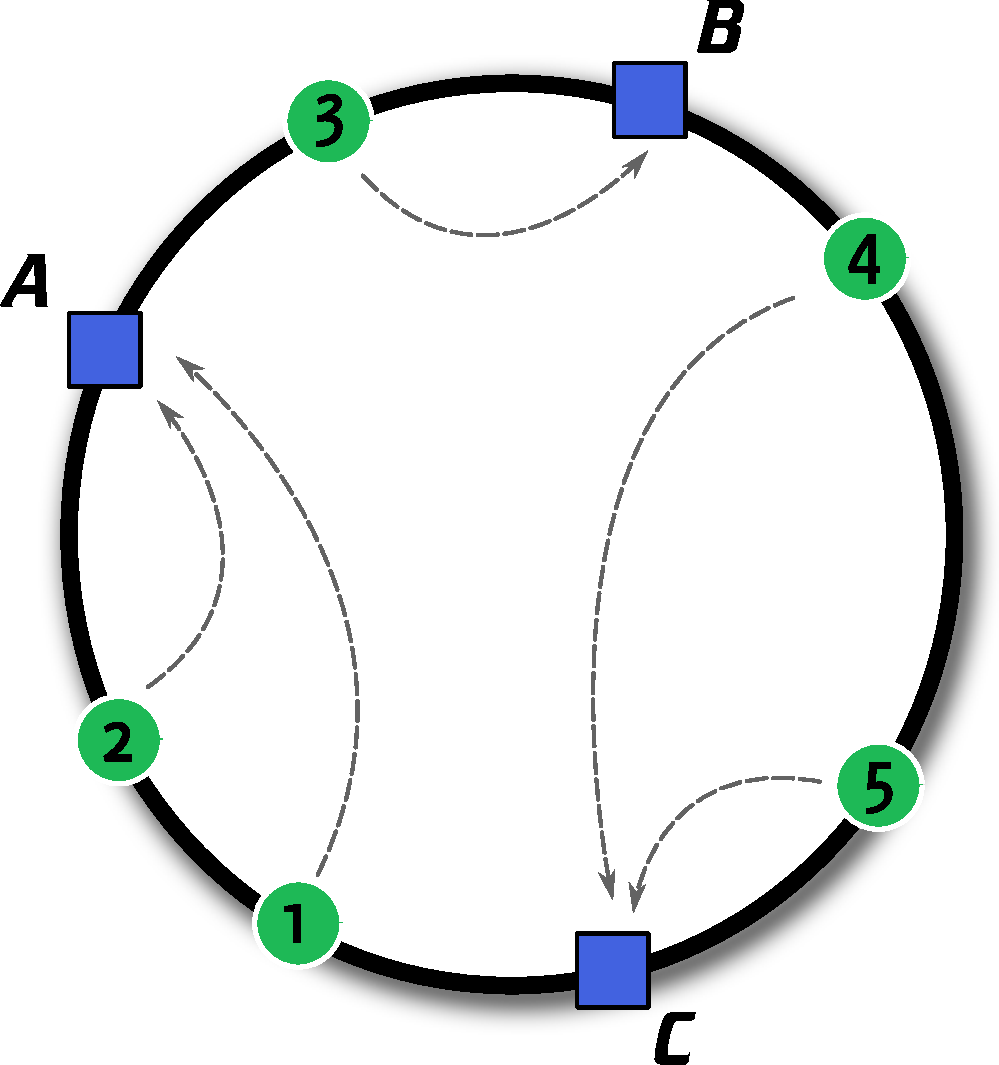
\includegraphics[width=0.95\textwidth]{img/consistent.pdf}
\end{minipage}
\begin{minipage}[b]{0.47\linewidth}
\centering
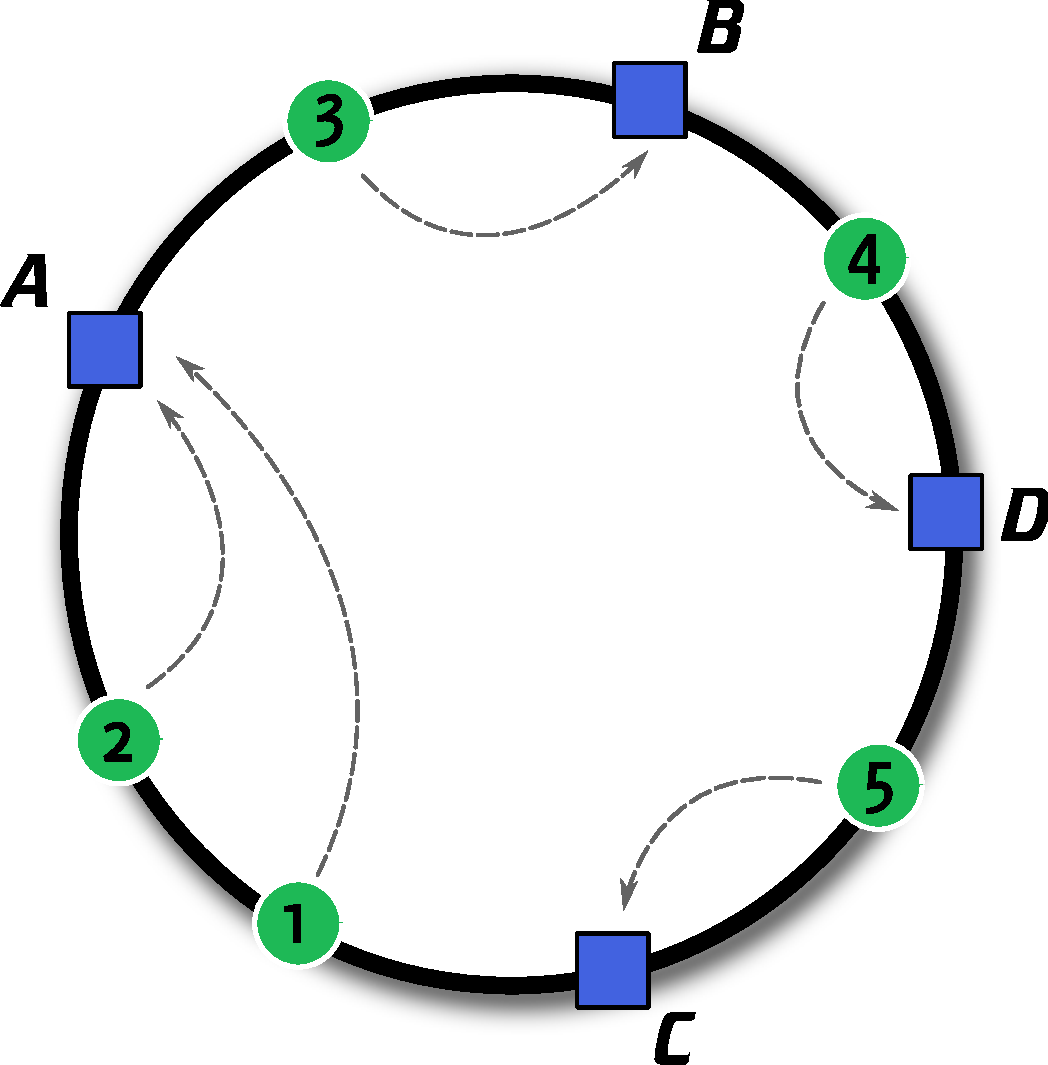
\includegraphics[width=0.95\textwidth]{img/consistent_2.pdf}
\end{minipage}
\caption{Idea \textit{Consistent Hashing}. Zasoby, reprezentowane przez zielone punkty, oraz serwery \keszujace\s (kwadraty) mapowane są na punkty na okręgu o jednostkowym obwodzie. Każdy serwer jest odpowiedzialny za obsługę zasobów znajdujących się pomiędzy jego punktem i punktem jego poprzednika. Dodanie nowego serwera $D$ powoduje wyłącznie zmianę przydziału zasobu $4$.}
\label{fig_consistent_hashing}
\end{figure}

W praktyce, przesłanie informacji dotyczących zmian serwerów do wszystkich klientów byłoby bardzo kosztowne, ale sytuacja, w której klienci mają różne ,,widoki'' (wiedzą tylko o pewnym podzbiorze serwerów) systemu nie stanowi problemu po wprowadzeniu prostej modyfikacji. Zauważmy, że może dojść do sytuacji, w której jeden z serwerów, z powodu niepełnej wiedzy klientów, będzie obsługiwał więcej żądań od pozostałych. W celu rozwiązania nierównego obciążenia autorzy zaproponowali stworzenie wirtualnych kopii serwerów, tzn. każdy z nich zmapowany jest nie do jednego, lecz kilku punktów na okręgu. Dzięki temu zagwarantowane jest równomierne przyporządkowanie zasobów do serwerów \cite{karger1999web}.

Pomimo, że pierwotną motywacją powstania \textit{Consistent Hashing} był problem \keszowania\s zasobów internetowych, schemat znalazł zastosowanie w innych obszarach. W szczególności, leży on u podstaw rozproszonych tablic haszujących, które omówione są w rozdziale \ref{sect_dht}.

\section{Rozproszone tablice haszujące (DHT)}
\label{sect_dht}
Rozproszone tablice haszujące (ang. \textit{Distributed Hash Tables}, DHT) to systemy pozwalające na przechowywanie par \textit{(klucz, wartość)}, podobnie jak zwykłe tablice haszujące, w dynamicznej sieci zbudowanej z uczestniczących węzłów (\textit{peer-to-peer}). Odpowiedzialność za przetrzymywanie mapowania kluczy do wartości jest podzielona pomiędzy węzłami, w taki sposób aby zmiany w liczbie uczestników nie powodowały reorganizacji systemu. Dodatkowo rozproszone tablice haszujące oferują efektywne wyszukiwanie kluczy w systemie.

Początkowe badania nad DHT były motywowane istniejącymi systemami peer-to-peer, oferującymi głównie możliwość dzielenia się plikami, np. \textit{Napster}, \textit{gnutella} i \textit{Freenet}. Sieci te w różnych sposób realizowały wyszukiwanie zasobów, ale każdy z nich miał swoje wady. \textit{Napster} korzystał z centralnego katalogu, do którego każdy serwer wysyłał swoją listę plików i który zarządzał wyszukiwaniem plików. W \textit{gnutelli} w celu odnalezienia zasobu, zapytanie wysyłane było do każdego węzła w sieci, co skutkowało mniejszą szybkością i mnóstwem przesyłanych wiadomości. W przypadku sieci \textit{Freenet}, znajdowanie klucza odbywało się za pomocą heurystycznej metody, która nie zapewniała, że klucz zostanie znaleziony.

Idea rozproszonych tablic haszujących ma na celu rozwiązanie wszystkich przedstawionych problemów:
\begin{itemize}
  \item w pełni rozproszony, skalowalny system; brak centralnego zarządzania,
  \item odporność na awarie węzłów,
  \item deterministyczny algorytm routingu, z dowiedzioną poprawnością, pozwalający na efektywne wyszukiwanie. 
\end{itemize} 

Jedną z pierwszy sieci DHT, bazującej na schemacie \textit{Consistent Hashing} jest \textit{Chord}, opisany w rozdziale \ref{sect_dht_chord}.

\subsection{Chord}
\label{sect_dht_chord}
TODO: Opis chorda jako zastosowanie Consistent Hashing

\subsection{Pastry}
TODO: Opis pastry w celu porównania Squirrela?
 
\subsection{Kademlia}
TODO: Opis Kademli\cite{maymounkov2002kademlia}: Routing, Asynchroniczność wywołań routingu - aspekty praktyczne.

\section{Rozproszony \kesz\s z użyciem DHT}

\subsection{Poprzednie prace}
TODO: Squirrel p2p web cache \cite{iyer2002squirrel}

\subsection{}
TODO: Opis połączenia keszowania z DHT - zastosowanie w celu realizacji pierwotnych idei. 
TODO: Zmiany w sieci w stosunku do ,,tamtych czasów'' :)
TODO: Opis efektu slashdot (przykłady stron w stylu reddit, wykop, etc)

\section{Analiza różnych metod cachowania}
TODO:
Cache wielopoziomowy:
\begin{enumerate}
  \item w pamięci,
  \item na dysku,
  \item w sieci P2P (te dane również w pamięci, na dysku)
\end{enumerate}
Różne strategie przechodzenia między poziomami.

\section{Testy}
\subsection{Spreparowane dane}


\subsection{Wdrożenie}
TODO: testy opóźnień?

\section{Implementacja}
\subsection{Wybór technologii}
Tutaj próby zrobienia tego w JS jako plugin do przeglądarki.
\subsection{Biblioteki}
Twisted, Entangled.
\subsection{Instalacja i uruchomienie}


\bibliographystyle{plain}

\bibliography{document}

\end{document}